% Full instructions available at:
% https://github.com/elauksap/focus-beamertheme

\documentclass{beamer}
\usetheme[numbering=progressbar]{focus}
\usepackage{tikz}
\usetikzlibrary{positioning}
\usetikzlibrary{shapes,arrows}
\usepackage{transparent}
\usepackage{fancyvrb}
\usepackage{listings}
\definecolor{main}{RGB}{47, 161, 219}
%\definecolor{textcolor}{RGB}{128, 128, 128}
\definecolor{background}{RGB}{240, 247, 255}
\definecolor{textcolor}{RGB}{85, 87, 83}
\title{D4 Project}
\subtitle{Revamping Passive SSL with D4}
\author{Jean-Louis Huynen}
\titlegraphic{
\includegraphics[width=140pt]{d4-logo.pdf}}
\institute{Team CIRCL \\ \url{https://www.d4-project.org/}}
\date{20190329}
 \lstset{%
        language=bash,
        backgroundcolor=\color{gray!25},
        basicstyle=\ttfamily,
        breaklines=true,
        columns=fullflexible
    }
\begin{document}

\begin{frame}
    \maketitle
\end{frame}
       
\begin{frame}
        \frametitle{A passive SSL fingerprinter}
        CSIRT's rationale for collecting TLS handshakes:
        \begin{itemize}
          \item Pivot on additional data points
          \item Find owners of IP addresses
          \item Detect usage of CIDR blocks
          \item Detect vulnerable systems
          \item Detect compromised services
        \end{itemize}
\end{frame}

\begin{frame}
  \frametitle{Objectives}

        History of links between:
        \begin{itemize}
          \item x509 certificates (And therefore their fields) 
          \item Ports
          \item IP address
          \item Client (ja3)
          \item Server (ja3s)
        \end{itemize}
\end{frame}
 
\begin{frame}
        \frametitle{Problem statement}
        \begin{itemize}
          \item CIRCL already offers a similar service based on SSLDump
          \item SSLDump needs some love - maintaining it is hard
          \item Alternatives do not span the entire TLS Handshake (Salesforce's ja3)
          \item TCP reassembly is not an easy problem to solve (Cloudfare uses tshark)
        \end{itemize}
\end{frame}

\begin{frame}
        \frametitle{sensor-d4-tls-fingerprinting}
        Main features:
        \begin{itemize}
          \item Take over SSLDump's duty
          \item written in Golang 
          \item uses Go packet for tcp reassembly and spans whole handshake
          \item ja3, ja3s, certificates, ip src / dst, port src / dst, TLSH
        \end{itemize}
        Current caveats:
        \begin{itemize}
          \item Support for TLS 1.3 pending
          \item Reassembly requires RAM
        \end{itemize}
\end{frame}

\begin{frame}
        \frametitle{sensor-d4-tls-fingerprinting}
        \begin{columns}
            \begin{column}{0.5\textwidth}
              \begin{center}
                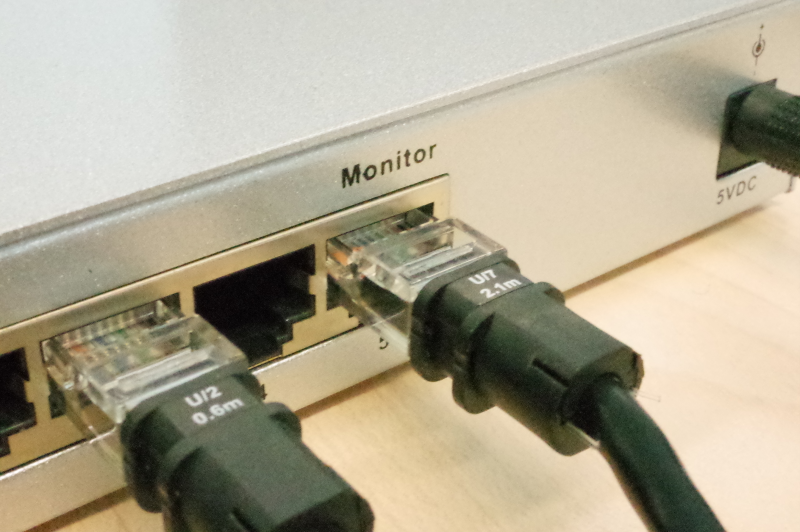
\includegraphics[scale=0.2]{../../informal-preso/0-intro-banana/monitor.png}
              \end{center}
            \end{column}
            \begin{column}{0.5\textwidth} 
              \begin{center}
                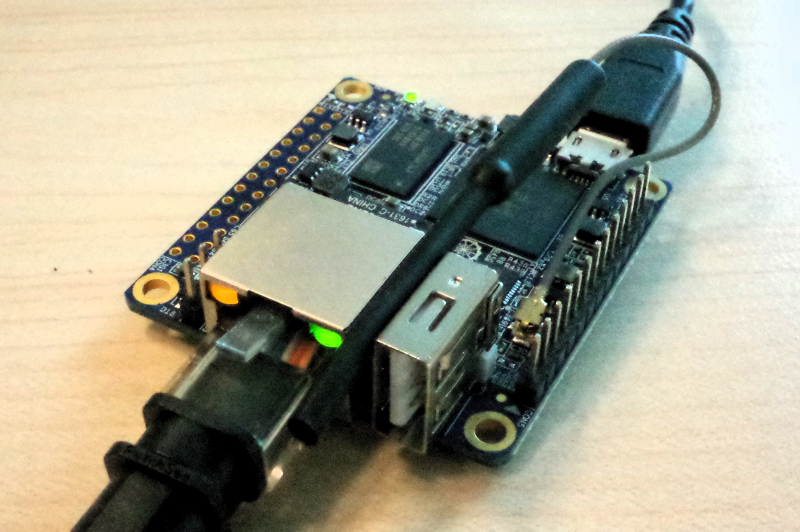
\includegraphics[scale=0.2]{../../informal-preso/0-intro-banana/orangepi.png}
              \end{center}
            \end{column}
          \end{columns}
          \hspace{20pt}
          \begin{itemize}
            \item 1 desktop monitored during 15 days
            \item 3327 TLS sessions fingerprinted
            \item 600 unique certificates collected
          \end{itemize}
\end{frame}

\begin{frame}
        \frametitle{sensor-d4-tls-fingerprinting - collectoin}

  \begin{lstlisting}
./d4-tlsf-amd64 -r|-i [-w -j -d -mbpc -mbpt -v] 
\end{lstlisting}



\begin{tabular}{l|l}
Options & Explanations\\
\hline
  -r & read pcap file\\
  -i & read from the interface \\
  -w & dump certificates to folder\\
  -j & write TLS session JSON descriptions to folder\\
  -mbcp & max buffered pages per connection (16) \\
  -mbpt & max total buffered pages (1024) \\
  -d & debug \\
  -v & verbose
\end{tabular}

\vspace{.8cm}
Available on the D4 project's github page\footnote{\url{github.com/D4-project/sensor-d4-tls-fingerprinting}}.
Depends on libpcap.

\end{frame}


\begin{frame}
        \frametitle{sensor-d4-tls-fingerprinting - d4 client} 
        \begin{lstlisting}
./d4-tlsf-amd64 -i eth0 | ./d4-amd64 -c conf.crq
\end{lstlisting}
        \vspace{.8cm}
        D4 server requires a meta-header in order to accept this data:
        \input{metaheader.json}
\end{frame}

\begin{frame}
        \frametitle{sensor-d4-tls-fingerprinting - d4 worker} 
        \begin{lstlisting}
    def __init__(self, uuid, json_file):
        super().__init__(uuid, json_file)
        self.set_rotate_file_mode(False)

    def process_data(self, data):
        self.reconstruct_data(data)

    def handle_reconstructed_data(self, data):
        ...
\end{lstlisting}
\end{frame}


\begin{frame}
\frametitle{Get in touch if you want to join the project, host a sensor or contribute}
\begin{itemize}
\item Collaboration can include research partnership, sharing of collected streams or improving the software.
\item Contact: info@circl.lu
\item \url{https://github.com/D4-Project} -  \url{https://twitter.com/d4_project}
\end{itemize}
\end{frame}


\end{document}
